\documentclass[11pt,oneside]{report}
\usepackage[letterpaper,left=0.89in,right=0.85in,top=0.87in,bottom=0.88in,headheight=17pt]{geometry}
\usepackage[T1]{fontenc}
\usepackage[utf8]{inputenc}
% pdfLaTeX-only typography (migrated from fontspec): Linux Libertine (roman)
% via the Type 1 "libertine" package, Lato as the sans family; DejaVu Sans
% Mono keeps its original 0.86 scaling.
\usepackage[rm]{libertine}
\usepackage[defaultsans]{lato}
\usepackage[scaled=0.86]{DejaVuSansMono}
\usepackage{microtype}
\usepackage[table]{xcolor}
\definecolor{navy}{HTML}{102A43}
\definecolor{cyan}{HTML}{0E7490}
\definecolor{teal}{HTML}{0F766E}
\definecolor{muted}{HTML}{52667B}
\definecolor{ice}{HTML}{E9F1F5}
\definecolor{ink}{HTML}{1D2A39}
\definecolor{gold}{HTML}{E5AF48}
\definecolor{linegray}{HTML}{D4E1E9}
\usepackage[most]{tcolorbox}
\usepackage{tabularx,longtable,booktabs,array,multirow}
\usepackage{ragged2e}
\usepackage{enumitem}
\usepackage{tikz}
\usetikzlibrary{positioning,arrows.meta,shapes.geometric,fit,backgrounds,calc}
\usepackage{graphicx}
\usepackage[cache=false]{minted}
\setminted{fontsize=\footnotesize,breaklines=true,breakanywhere=true,frame=single,framesep=5pt,rulecolor=\color{linegray}}
\usepackage{fancyhdr}
\usepackage{titlesec}
\usepackage{needspace}
\usepackage{amsmath}
\usepackage{hyperref}
\hypersetup{colorlinks=true,linkcolor=cyan,urlcolor=cyan,citecolor=teal,pdftitle={Open-Source Enterprise Security Platform},pdfauthor={Enterprise Security Architecture Research}}
\urlstyle{same}
\setlength{\parskip}{5.0pt}
\setlength{\parindent}{0pt}
\setlength{\emergencystretch}{3em}
\renewcommand{\arraystretch}{1.19}
\setcounter{tocdepth}{2}
\setcounter{secnumdepth}{3}
\titleformat{\chapter}[display]{\sffamily\bfseries\color{navy}}{\large\color{cyan} PART \thechapter}{4pt}{\Huge}[\vspace{5pt}\color{gold}\titlerule]
\titlespacing*{\chapter}{0pt}{-8pt}{17pt}
\titleformat{\section}{\large\sffamily\bfseries\color{navy}}{\thesection}{0.65em}{}
\titleformat{\subsection}{\normalsize\sffamily\bfseries\color{cyan}}{\thesubsection}{0.65em}{}
\pagestyle{fancy}\fancyhf{}\fancyhead[L]{\sffamily\small\color{muted} OPEN-SOURCE ENTERPRISE SECURITY}\fancyhead[R]{\sffamily\small\color{muted} OCT 2026}\fancyfoot[L]{\sffamily\footnotesize\color{muted} RESEARCH EDITION \textbullet\ 2026-10-12}\fancyfoot[R]{\sffamily\footnotesize\color{muted} \thepage}
\renewcommand{\headrulewidth}{0.3pt}\renewcommand{\footrulewidth}{0pt}
\fancypagestyle{plain}{\fancyhf{}\fancyfoot[R]{\sffamily\color{muted}\thepage}\renewcommand{\headrulewidth}{0pt}}
\newtcolorbox{insight}[1][]{colback=ice,colframe=cyan!60,boxrule=.6pt,arc=1.5mm,left=3.3mm,right=3.3mm,top=2.3mm,bottom=2.3mm,breakable,#1}
\newtcolorbox{caution}[1][]{colback=gold!8,colframe=gold!85!black,boxrule=.6pt,arc=1.5mm,left=3.3mm,right=3.3mm,top=2.3mm,bottom=2.3mm,breakable,#1}
\newcommand{\term}[1]{\textsf{\textbf{#1}}}
\newcommand{\data}[1]{{\sffamily\color{cyan}\bfseries #1}}
\newcommand{\status}[1]{\textsf{\footnotesize #1}}
\newcolumntype{Y}{>{\RaggedRight\arraybackslash}X}
\newcolumntype{P}[1]{>{\RaggedRight\arraybackslash}p{#1}}
\begin{document}
\begin{titlepage}
\pagecolor{navy}\color{white}
\vspace*{1.05in}
{\sffamily\bfseries\fontsize{12}{15}\selectfont REFERENCE ARCHITECTURE \textbullet\ RESEARCH CATALOGUE}\par
\vspace{0.18in}
{\color{gold}\rule{0.82\textwidth}{2.5pt}}\par
\vspace{0.48in}
{\sffamily\bfseries\fontsize{35}{41}\selectfont Open-Source\\Enterprise Security\\Platform}\par
\vspace{0.27in}
{\sffamily\fontsize{17}{23}\selectfont Capability model, tool qualification, architecture,\\engineering blueprint and implementation roadmap}\par
\vfill
{\sffamily\bfseries\large ENGINEERING RESEARCH EDITION}\par
\vspace{0.15in}
{\sffamily\normalsize Baseline: ImmunitySec's 28-category directory and independent upstream research}\par
\vspace{0.23in}
{\sffamily\normalsize 12 October 2026 \textbullet\ Decision-support document \textbullet\ Evidence-labeled}\par
\vspace{0.3in}
\end{titlepage}
\nopagecolor\color{ink}
\pagenumbering{roman}
\begin{insight}
\textbf{Research status.} This is an evidence-labeled architectural assessment, \emph{not} a claim that all 337 advertised directory profiles or all 140 cataloged projects received a full 30-field upstream audit. The directory's 28 category pages were opened; 24 projects were reviewed against upstream material; 116 additional entries remain discovery candidates. No proposed software is production-approved without license, security, deployment, and integration gates.
\end{insight}
\tableofcontents
\clearpage
\pagenumbering{arabic}

\chapter{Executive security tool strategy}
\section{Executive decision}
Adopt a \term{capability-first, open-source-first} program that uses open-source components where they provide sufficient assurance, while recognizing that identity, backup, patch management, monitoring, and governance must be operational processes rather than products alone. The platform should begin with authoritative ownership and inventory, standardize software evidence and findings, and scale detection, response, cloud, and specialist testing only as the threat model justifies.

\begin{insight}
\textbf{Recommended architectural backbone}\par
\textbf{Inventory / ownership} $\rightarrow$ \textbf{telemetry and scanning} $\rightarrow$ \textbf{normalization / deduplication} $\rightarrow$ \textbf{risk-aware remediation} $\rightarrow$ \textbf{evidence and reporting}.\par
For organizations that build software, complement this backbone with mandatory secrets detection, SAST, dependency analysis, SBOM generation, and artifact verification in CI/CD.
\end{insight}

\section{Decision principles}
\begin{enumerate}[leftmargin=1.6em,itemsep=3pt]
\item Fund security \emph{outcomes}, not the number of tools deployed.
\item Prefer upstream-maintained, OSI-licensed components and verify editions, plug-ins, feeds, rule sets, and commercial features separately.
\item Reuse existing reliable identity and platform services instead of deploying a second identity provider or log lake by default.
\item Introduce a custom integration service only when native imports, exports, APIs, and platform workflows cannot satisfy a documented requirement.
\item Build a single asset-to-finding-to-owner-to-remediation trace, but keep assets, vulnerabilities, findings, incidents, and risks as distinct entities.
\item Gate intrusive assessments behind explicit written authorization; never treat catalog discovery as permission to test third-party infrastructure.
\end{enumerate}

\section{The minimum viable security platform}
A credible baseline requires an accountable security owner, current asset and application inventory, an identity service with multifactor authentication, managed endpoint updates, off-site recoverable backups, centralized security-relevant logs, recurring vulnerability assessment and remediation, incident escalation, and tested recovery. Software development organizations also need code and dependency scanning. This minimum is an \emph{outcome baseline}, not a fixed software bill of materials.

\section{Source provenance and confidence}
Evidence classes used throughout: \textbf{D} = directory observation, \textbf{U} = upstream documentation or repository checked, \textbf{A} = architecture recommendation, \textbf{E} = illustrative engineering estimate, and \textbf{Q} = pending qualification. An upstream-reviewed project is not necessarily version-verified, integrated, benchmarked, or security-accredited.

\begin{caution}
\textbf{Notable licensing boundary.} ImmunitySec identifies Nmap's NPSL as non-OSI-approved\cite{immunity,nmap}. It is not part of the strict OSS shortlist despite its practical utility. Commercial Burp Suite is likewise not open-source; OSS ZAP is evaluated for the DAST capability. Elastic's upstream distribution requires file/feature license scoping rather than a blanket OSS claim. See the primary directory and upstream license references.
\end{caution}

\chapter{Directory discovery and coverage}
\section{Scope and integrity of website findings}
The source directory advertises \textbf{337 tool profiles in 28 categories}\cite{immunity} as accessed on 2026-10-12. All 28 landing pages were opened for category-level reconnaissance. Published per-category counts add to 337, but individual tool profile completeness, uniqueness across taxonomy versions, individual license values, releases, and all tool claims have \emph{not} been audited. Category-level labels below express enterprise deployment judgments, not the source website's classifications.

\begin{longtable}{P{0.30\textwidth}P{0.08\textwidth}P{0.18\textwidth}P{0.31\textwidth}}
\toprule \textbf{Directory category} & \textbf{Count} & \textbf{Criticality} & \textbf{Enterprise outcome / examples}\\ \midrule\endfirsthead
\toprule \textbf{Directory category} & \textbf{Count} & \textbf{Criticality} & \textbf{Outcome / examples}\\ \midrule\endhead

AI Security Tools & 10 & Conditional & LLM and agent assurance; garak; PyRIT; ART \\
Application Security Tools & 23 & Conditional & SAST, DAST, API testing; ZAP; Semgrep; Gitleaks \\
Binary Exploitation & 7 & Specialist & Low-level security research; pwntools; ROPgadget \\
Cloud Security Tools & 20 & Conditional & Cloud and workload posture; Prowler; Trivy; Falco \\
CTF \& Practice Labs & 16 & Specialist & Training and technical exercises; Juice Shop; DVWA \\
Data Security Software & 10 & Foundational & Encryption and sensitive-data control; Gitleaks; OpenBao \\
Digital Forensics & 12 & Conditional & Host and memory investigations; Velociraptor; Volatility 3 \\
Email Security Software & 13 & Foundational & Email authentication and filtering; Rspamd; SpamAssassin \\
Fuzzing & 10 & Specialist & Input robustness testing; AFL++; libFuzzer \\
GRC Software & 11 & Foundational & Risk, policy and compliance evidence; OpenSCAP; compliance-trestle \\
Honeypot \& Deception Tools & 8 & Conditional & High-signal decoys; Cowrie; T-Pot \\
IAM Tools & 10 & Foundational & Authentication and secrets; Keycloak; OpenBao \\
Malware Analysis Tools & 12 & Specialist & Malware triage and classification; YARA; capa \\
Mobile Security Software & 8 & Conditional & Mobile app assessment; MobSF; Frida \\
Network Monitoring Tools & 5 & Conditional & Packet and flow analysis; Zeek; Suricata; Arkime \\
Network Security Tools & 13 & Foundational & Firewalls and remote access; OPNsense; WireGuard \\
Open Source Intelligence Tools & 19 & Specialist & External exposure and enrichment; Amass; SpiderFoot \\
OT/ICS Security Tools & 6 & Conditional & Industrial asset visibility; GRASSMARLIN; Malcolm \\
Password Cracking & 7 & Specialist & Authorized credential auditing; John the Ripper; hashcat \\
Penetration Testing Tools & 21 & Specialist & Authorized application and network testing; ZAP; Metasploit \\
Phishing Simulation Tools & 5 & Conditional & Awareness assessment; GoPhish \\
Red Teaming Tools & 11 & Specialist & Purple team validation; Atomic Red Team; CALDERA \\
Reverse Engineering & 12 & Specialist & Program analysis; Ghidra; radare2 \\
SIEM Tools & 29 & Conditional & Centralized detection and case workflows; Wazuh; Sigma; OpenSearch \\
Software Composition Analysis Tools & 12 & Conditional & SBOM, dependencies, provenance; Syft; Grype; Dependency-Track \\
Threat Intelligence Tools & 9 & Conditional & Enrichment and sharing; MISP; OpenCTI \\
Vulnerability Scanning & 8 & Foundational & Infrastructure exposure discovery; Greenbone; Trivy \\
Wireless \& RF Security & 10 & Specialist & Wireless/RF validation; Kismet; Wireshark \\
\bottomrule
\end{longtable}
\textbf{Classification rule.} \emph{Foundational} means the outcome is broadly essential but the named category may be implemented by a provider service or an existing tool; \emph{Conditional} means sector, architecture, maturity, or threat exposure determines applicability; \emph{Specialist} implies laboratory, assessment, forensics, or focused expertise. Offensive/testing categories are not routine production agents.

\section{Coverage and evidence ledger}

\noindent\begin{tabularx}{\textwidth}{lXr}
\toprule Measure & Meaning & Count\\\midrule
Source categories located/opened & Category landing pages inspected & 28\\
Published category profiles & Website-reported sum; not independently audited & 337\\
Upstream-reviewed projects & Official repository and/or upstream licensing material examined & 24\\
Additional discovery leads & Project candidates with qualifications outstanding & 116\\
Total registry entries & Non-duplicated research entries in supplied JSON/CSV & 140\\
Profiles individually audited & Exhaustive 30-field profile audit performed & 0\\
Production-approved deployments & Environment-specific acceptance and security signoff & 0\\
\bottomrule
\end{tabularx}
\par\textit{Limitations:} sitemap and robots.txt could not be independently retrieved through the research interface; this does not authorize aggressive crawling. Release dates, software requirements, community health, and many integration assertions remain explicitly unverified in the registry. Category landing-page observations must not be conflated with official upstream product verification.

\section{Enterprise capability gaps beyond the directory}
The directory is strongest for security software discovery; a complete enterprise program additionally requires CMDB/asset ownership, patch deployment, certificate life cycle, business continuity, third-party governance, encrypted backup/restore validation, ITSM, data ownership and retention, legal obligations, and capacity planning. These capabilities are included because a company's security control environment cannot be represented exclusively by offensive security and detection utilities.

\chapter{Security capability model}
\section{Control orientation and applicability}
NIST CSF 2.0 supplies the top-level functions\cite{nist}; the CIS Controls v8.1 references\cite{cis} identify relevant \emph{control families}, not audited safeguard-level crosswalks. IG labels below are \emph{planning approximations}, not a definitive claim that a specific CIS Safeguard belongs to the indicated group. Every organization should start from IG1, expand through IG2, and apply IG3 safeguards based on its risk context. Detailed licensing of CIS materials should be respected.
\small
\begin{longtable}{P{0.095\textwidth}P{0.125\textwidth}P{0.25\textwidth}P{0.21\textwidth}P{0.18\textwidth}}
\toprule ID & CSF & Capability & CIS planning reference & Owner\\\midrule\endfirsthead
\toprule ID & CSF & Capability & CIS reference & Owner\\\midrule\endhead

CAP-01 & Govern & Policy and risk & CIS 17; IG1 start & GRC lead \\
CAP-02 & Identify & Hardware/network inventory & CIS 1; IG1 & Infrastructure \\
CAP-03 & Identify & Software and application inventory & CIS 2; IG1 & IT / AppSec \\
CAP-04 & Protect & Secure configurations & CIS 4; IG1 & Platform \\
CAP-05 & Protect & Identity and MFA & CIS 5,6; IG1 & IAM \\
CAP-06 & Protect & Secrets and PKI & CIS 3,6; IG1+ & IAM/Platform \\
CAP-07 & Protect & Patch and update lifecycle & CIS 7; IG1 & IT Operations \\
CAP-08 & Protect & Backup and recovery & CIS 11; IG1 & SRE/DR \\
CAP-09 & Protect & Email and DNS protection & CIS 9,12; IG1+ & Messaging \\
CAP-10 & Detect & Endpoint and log telemetry & CIS 8,10; IG1+ & SOC/IT \\
CAP-11 & Detect & Network security monitoring & CIS 12,13; IG2+ & NetSec/SOC \\
CAP-12 & Identify & Vulnerability scanning & CIS 7; IG1+ & Vuln Mgmt \\
CAP-13 & Identify & Exposure prioritization & CIS 7; IG2+ & Vuln Mgmt \\
CAP-14 & Protect & Secure SDLC and SAST & CIS 16; IG2+ & AppSec \\
CAP-15 & Protect & DAST, API tests, fuzzing & CIS 16,18; IG2+ & AppSec/QA \\
CAP-16 & Identify & SBOM and SCA & CIS 2,16; IG2+ & AppSec/Supply Chain \\
CAP-17 & Protect & Provenance and artifact signing & CIS 16; IG2+ & Platform/Release \\
CAP-18 & Identify & Cloud posture & CIS 4,15; IG2+ & CloudSec \\
CAP-19 & Protect & Kubernetes policy/runtime & CIS 4,13,16; IG2+ & Platform/K8s \\
CAP-20 & Protect & Data inventory and encryption & CIS 3; IG1+ & Data Security \\
CAP-21 & Detect & SIEM and detection engineering & CIS 8,13; IG2+ & SOC \\
CAP-22 & Respond & Casework and DFIR & CIS 17; IG1+ & IR/SOC \\
CAP-23 & Identify & Threat intelligence & CIS 13,17; IG2+ & CTI/SOC \\
CAP-24 & Recover & Continuity and restore tests & CIS 11,17; IG1 & BCM/SRE \\
CAP-25 & Govern & Third-party risk & CIS 15; IG2+ & GRC/Vendor \\
CAP-26 & Identify & AI system assurance & CIS 16; conditional & AI/AppSec \\
CAP-27 & Identify & OT/ICS monitoring & CIS 1,13; conditional & OT Sec \\
CAP-28 & Detect & Adversary validation & CIS 18; IG2+ & Purple team \\
\bottomrule\end{longtable}\normalsize
\section{Operational contracts: inputs, outputs and prerequisites}
\footnotesize
\begin{longtable}{P{0.10\textwidth}P{0.26\textwidth}P{0.27\textwidth}P{0.25\textwidth}}
\toprule ID & Input & Expected output and workflow & Prerequisites\\\midrule\endfirsthead
\toprule ID & Input & Output / workflow & Prerequisites\\\midrule\endhead

CAP-01 & Control owners + risks & Approved policies and exceptions & Executive risk mandate \\
CAP-02 & Discovery, DHCP, CMDB & Owned asset records & Discovery credentials \\
CAP-03 & Package, repo, app data & Owned portfolio + SBOM links & CAP-02 \\
CAP-04 & Baseline + host configs & Hardened drift alerts & CAP-02 \\
CAP-05 & Identities, groups, entitlements & SSO/MFA and audit events & Identity owners \\
CAP-06 & Certificates, secrets, keys & Rotation and secure issuance & CAP-05 \\
CAP-07 & Assets, software, advisories & Installed, verified updates & CAP-02/03 \\
CAP-08 & RPO/RTO, protected data & Verified restorable copies & Asset and data owners \\
CAP-09 & Domain / mail signals & Filtering and auth telemetry & DNS ownership \\
CAP-10 & Host events, audit logs & Actionable detections & CAP-02/05 \\
CAP-11 & Mirrored traffic, flow & NDR events and context & Network TAP/permissions \\
CAP-12 & Authorized scan scope & Asset-linked findings & CAP-02 \\
CAP-13 & CVE, EPSS, KEV, context & Ranked owner-assigned work & CAP-12 \\
CAP-14 & Source and build metadata & CI findings + prevention & CI + repos \\
CAP-15 & Safe staging apps & Confirmed technical findings & Authorized test environments \\
CAP-16 & Artifacts, manifests & Inventory and vuln context & CAP-03/14 \\
CAP-17 & Build metadata and keys & Validated attestations & CAP-06/16 \\
CAP-18 & Read-only cloud inventory & Misconfiguration issues & Cloud account inventory \\
CAP-19 & K8s audit, images, events & Admission, runtime alerts & CAP-18 \\
CAP-20 & Data classes, stores & Approved access/encryption & Data ownership \\
CAP-21 & Normalized security events & Quality alerts and coverage & CAP-10 \\
CAP-22 & Detections, evidence & Tracked incidents and artifacts & CAP-21 \\
CAP-23 & IOCs, STIX, ATT\&CK & Validated enrichments & Use cases and sources \\
CAP-24 & RTO/RPO, backups & Proven recovery outcomes & CAP-08 \\
CAP-25 & Supplier register, contracts & Critical vendor tracking & CAP-01 \\
CAP-26 & LLM apps and tools & Behavioral eval reports & AI system inventory \\
CAP-27 & OT topology, passive data & Safe asset visibility & Safety approvals \\
CAP-28 & Approved test cases & Measured detection gaps & CAP-21/22 \\
\bottomrule\end{longtable}\normalsize
\section{Specialized engineering framework overlays}

\noindent\begin{tabularx}{\textwidth}{P{0.28\textwidth}Y}
\toprule Overlay & How the platform uses it\\\midrule
NIST SP 800-218 (SSDF) & Secure-development practices and CI evidence across repository, build and deployment lifecycles; not a replacement for risk governance.\\
OWASP SAMM and ASVS & Maturity improvement and verifiable application security requirements; mapping requires version- and application-specific assessment.\\
MITRE ATT\&CK & Detection coverage and adversary emulation hypothesis; ATT\&CK techniques are not equivalent to vulnerabilities.\\
MITRE ATLAS & AI threat-informed evaluation for deployed AI/agent systems; assess model access and tool-permission risks.\\
CISA KEV and FIRST EPSS & Exploitation signals for triage; KEV presence is binary catalogue evidence, while EPSS is a predicted 30-day exploitation probability, not guaranteed impact.\\
OSCAL, SARIF, CycloneDX, SPDX & Typed interchange formats for compliance evidence, source findings and software inventories; preserve original schemas and provenance.\\
\bottomrule
\end{tabularx}

\chapter{Tool qualification and selection}
\section{Open-source gate and legal review}
\begin{enumerate}[leftmargin=1.6em]
\item Confirm an official upstream repository and the released artifact's exact source license, including code, UI, rules, plug-ins, images, feeds and dependencies.
\item Require an OSI-approved license for the proposed \emph{deployed component}; separately identify open-core and commercially gated features.
\item Review GPL/LGPL/AGPL/MPL obligations with legal counsel where source distribution, linking, network access, or modified services may trigger obligations.
\item Evaluate security policy, release signatures, maintenance responsiveness, upgrade trajectory, authentication, isolation and data-handling quality.
\item Demonstrate successful integration and restore before declaring production-ready.
\end{enumerate}
\section{Weighted screening model}
A repeatable scoring rubric uses a one-to-five ordinal scale (1 = weak or not evidenced; 3 = adequate for the reference context; 5 = strong and evidenced). Missing hard-gate evidence results in \term{hold}, not automatic approval. Weights are functional 25\%, maintenance 20\%, security 15\%, integration 15\%, operating cost 10\%, license suitability 10\%, and documentation 5\%. The model is \emph{comparative and scenario-dependent}; it is not a benchmark.
\[
S=0.25F+0.20M+0.15T+0.15I+0.10O+0.10L+0.05D,
\qquad 1 \le S \le 5.
\]
\begin{caution}
\textbf{Scoring integrity.} The matrix below expresses hypothetical architecture-fit screening judgments, not empirically verified throughput, support SLAs, or security efficacy. All scores must be revisited after a proof of concept and evidence-backed license review. Do not treat rank order as a procurement determination.
\end{caution}

\small
\begin{longtable}{P{0.22\textwidth}*{7}{>{\centering\arraybackslash}p{0.035\textwidth}}P{0.07\textwidth}P{0.15\textwidth}}
\toprule Project & F & M & T & I & O & L & D & \textbf{Score} & Fit rationale\\\midrule\endfirsthead
\toprule Project & F & M & T & I & O & L & D & Score & Rationale\\\midrule\endhead

Gitleaks & 5 & 4 & 4 & 5 & 5 & 5 & 4 & 4.60 & CI secrets checks \\
Syft & 5 & 4 & 4 & 5 & 5 & 5 & 4 & 4.60 & SBOM generation \\
Trivy & 5 & 4 & 4 & 5 & 4 & 5 & 4 & 4.50 & Unified developer-side scanner \\
restic & 5 & 4 & 4 & 4 & 5 & 5 & 4 & 4.45 & Encrypted backup \\
Keycloak & 5 & 4 & 4 & 5 & 3 & 5 & 4 & 4.40 & Identity provider if needed \\
Prowler & 5 & 4 & 4 & 4 & 4 & 5 & 4 & 4.35 & Cloud posture \\
Kyverno & 5 & 4 & 4 & 4 & 4 & 5 & 4 & 4.35 & Kubernetes policy \\
ZAP & 5 & 4 & 4 & 4 & 3 & 5 & 4 & 4.25 & DAST for authorized staging \\
Grype & 4 & 4 & 4 & 5 & 4 & 5 & 4 & 4.25 & Alternative package scanner \\
Dependency-Track & 5 & 4 & 4 & 4 & 3 & 5 & 4 & 4.25 & Portfolio SBOM analysis \\
DefectDojo & 5 & 4 & 4 & 4 & 3 & 5 & 4 & 4.25 & Finding workflows \\
OpenBao & 5 & 4 & 4 & 4 & 3 & 5 & 4 & 4.25 & Secrets management \\
Wazuh & 5 & 4 & 4 & 4 & 3 & 4 & 4 & 4.15 & Host-focused security operations \\
Semgrep OSS engine & 4 & 4 & 4 & 4 & 4 & 4 & 4 & 4.00 & Simple portable SAST, no proprietary features assumed \\
Falco & 4 & 4 & 4 & 4 & 3 & 5 & 4 & 4.00 & Runtime telemetry \\
Velociraptor & 5 & 4 & 4 & 3 & 3 & 4 & 4 & 4.00 & DFIR response \\
\bottomrule\end{longtable}\normalsize
\section{Selection and overlap decisions}

\noindent\begin{tabularx}{\textwidth}{P{0.25\textwidth}P{0.25\textwidth}Y}
\toprule Capability & Preferred / alternative & Architecture decision\\\midrule
Secrets scanning & Gitleaks / detect-secrets & Use one default scanner and a review process; treat true positives as credential incidents.\\
SAST & Semgrep OSS / language-specific analyzers & Select by language coverage and rule quality; clearly exclude proprietary analysis services.\\
DAST & ZAP / targeted manual testing & Isolate scanners in staging with explicit rate and authorization constraints.\\
Image CVEs & Trivy / Grype & One default CI gate; use a second engine only for independent validation.\\
SBOM portfolio & Syft + Dependency-Track & Generator and portfolio consumer are complementary, not duplicates.\\
Finding workflow & DefectDojo / existing ITSM & Reuse existing case ownership; avoid custom ticketing where imports work.\\
Secrets platform & OpenBao / provider-native KMS & KMS, secret stores and PKI fulfill different functions; do not deploy unnecessarily.\\
Endpoint detection & Wazuh / existing EDR & Avoid parallel agents without clear coverage and performance justification.\\
Network detection & Suricata + Zeek & Signature events and rich protocol logs can complement; telemetry cost may preclude both.\\
K8s policy & Kyverno / OPA Gatekeeper & Select one admission framework for shared policy ownership.\\
CTI & MISP / OpenCTI Community & Start with a use case and exchange obligations; CTI platforms are not mandatory for Tier 1.\\
\bottomrule
\end{tabularx}
\section{Disqualified, conditional or unresolved cases}
\textbf{Nmap:} Source-available/non-OSI under NPSL as identified by the directory; exclude from \emph{strict} open-source selection. \textbf{Burp Suite:} proprietary; exclude from OSS platform. \textbf{Elastic stack:} source and distribution include different licenses; require package-by-package review. \textbf{TheHive, Grafana, Giskard, authentik, Checkov, open-core vendors:} not rejected as unsuitable products, but production claims and the deployable-edition license must be verified. \textbf{Greenbone:} the C and Rust scanner components and vulnerability feeds have separate licensing and distribution considerations. \textbf{osquery:} multiple license files require component-level analysis. \textbf{OpenCTI:} Community Edition is distinct from licensed enterprise features.

\chapter{Open-source tool registry}
\section{Registry interpretation}
The complete registry is supplied as \texttt{tool\_catalog.csv} and \texttt{tool\_registry.json}. It contains 140 unique research records with explicit evidence states and structured placeholders for 39+ fields. The table below is a \emph{staged discovery index}, not a claim that all 140 entries are currently qualified as open source. \textbf{U} denotes an upstream-reviewed shortlist; \textbf{Q} denotes a candidate whose licensing, status, edition and operability require verification. For upstream-reviewed projects, exact version and deployment characteristics are still generally unverified.

\footnotesize
\begin{longtable}{P{0.10\textwidth}P{0.32\textwidth}P{0.22\textwidth}P{0.155\textwidth}P{0.055\textwidth}}
\toprule ID & Project & Domain & License lead & Stage\\\midrule\endfirsthead
\toprule ID & Project & Domain & License lead & Stage\\\midrule\endhead

TOOL-001 & ZAP & Application security & Apache-2.0 & U \\
TOOL-002 & Semgrep OSS engine & Application security & LGPL-2.1-only & U \\
TOOL-003 & Gitleaks & Application security & MIT & U \\
TOOL-004 & Trivy & Cloud and supply chain & Apache-2.0 & U \\
TOOL-005 & Syft & Supply chain & Apache-2.0 & U \\
TOOL-006 & Grype & Supply chain & Apache-2.0 & U \\
TOOL-007 & Dependency-Track & Supply chain & Apache-2.0 & U \\
TOOL-008 & DefectDojo & Vulnerability management & BSD-3-Clause & U \\
TOOL-009 & Keycloak & Identity & Apache-2.0 & U \\
TOOL-010 & OpenBao & Identity & MPL-2.0 & U \\
TOOL-011 & Wazuh & Detection and response & GPL-2.0-only WITH OpenSSL-exception* & U \\
TOOL-012 & Suricata & Network detection & GPL-2.0-only & U \\
TOOL-013 & Zeek & Network detection & BSD-style* & U \\
TOOL-014 & Prowler & Cloud security & Apache-2.0 & U \\
TOOL-015 & Falco & Cloud and supply chain & Apache-2.0 & U \\
TOOL-016 & Kyverno & Cloud and supply chain & Apache-2.0 & U \\
TOOL-017 & Cosign & Supply chain & Apache-2.0 & U \\
TOOL-018 & restic & Backup and recovery & BSD-2-Clause & U \\
TOOL-019 & MISP & Threat intelligence & AGPL-3.0-only* & U \\
TOOL-020 & OpenCTI Community & Threat intelligence & Apache-2.0* & U \\
TOOL-021 & Greenbone OpenVAS Scanner & Vulnerability management & GPL-2.0-only* & U \\
TOOL-022 & Velociraptor & Incident response & AGPL-3.0-only & U \\
TOOL-023 & Open Policy Agent & Governance and compliance & Apache-2.0 & U \\
TOOL-024 & osquery & Endpoint and inventory & Mixed Apache-2.0/GPL-2.0* & U \\
TOOL-025 & OpenSCAP & Governance and compliance & Not verified & Q \\
TOOL-026 & Compliance Trestle & Governance and compliance & Not verified & Q \\
TOOL-027 & Steampipe & Cloud security & Not verified & Q \\
TOOL-028 & Cloud Custodian & Cloud security & Not verified & Q \\
TOOL-029 & ScoutSuite & Cloud security & Not verified & Q \\
TOOL-030 & Checkov & Application security & Not verified & Q \\
TOOL-031 & Terrascan & Application security & Not verified & Q \\
TOOL-032 & Terratest & Application security & Not verified & Q \\
TOOL-033 & Bandit & Application security & Not verified & Q \\
TOOL-034 & Brakeman & Application security & Not verified & Q \\
TOOL-035 & SpotBugs & Application security & Not verified & Q \\
TOOL-036 & FindSecBugs & Application security & Not verified & Q \\
TOOL-037 & CodeQL CLI & Application security & Not verified & Q \\
TOOL-038 & detect-secrets & Application security & Not verified & Q \\
TOOL-039 & TruffleHog & Application security & Not verified & Q \\
TOOL-040 & Nuclei & Application security & Not verified & Q \\
TOOL-041 & SQLMap & Application security & Not verified & Q \\
TOOL-042 & ffuf & Application security & Not verified & Q \\
TOOL-043 & AFL++ & Fuzzing and binary & Not verified & Q \\
TOOL-044 & libFuzzer & Fuzzing and binary & Not verified & Q \\
TOOL-045 & Honggfuzz & Fuzzing and binary & Not verified & Q \\
TOOL-046 & boofuzz & Fuzzing and binary & Not verified & Q \\
TOOL-047 & Atheris & Fuzzing and binary & Not verified & Q \\
TOOL-048 & Ghidra & Fuzzing and binary & Not verified & Q \\
TOOL-049 & radare2 & Fuzzing and binary & Not verified & Q \\
TOOL-050 & pwntools & Fuzzing and binary & Not verified & Q \\
TOOL-051 & Volatility 3 & Incident response & Not verified & Q \\
TOOL-052 & Autopsy & Incident response & Not verified & Q \\
TOOL-053 & Plaso & Incident response & Not verified & Q \\
TOOL-054 & YARA & Incident response & Not verified & Q \\
TOOL-055 & capa & Incident response & Not verified & Q \\
TOOL-056 & Timesketch & Incident response & Not verified & Q \\
TOOL-057 & TheHive & Incident response & Not verified & Q \\
TOOL-058 & Cortex & Incident response & Not verified & Q \\
TOOL-059 & Shuffle & Incident response & Not verified & Q \\
TOOL-060 & StackStorm & Incident response & Not verified & Q \\
TOOL-061 & Arkime & Network detection & Not verified & Q \\
TOOL-062 & Wireshark & Network detection & Not verified & Q \\
TOOL-063 & tcpdump & Network detection & Not verified & Q \\
TOOL-064 & Malcolm & Network detection & Not verified & Q \\
TOOL-065 & Kismet & Network detection & Not verified & Q \\
TOOL-066 & ntopng & Network detection & Not verified & Q \\
TOOL-067 & OPNsense & Network security & Not verified & Q \\
TOOL-068 & WireGuard & Network security & Not verified & Q \\
TOOL-069 & NetBird & Network security & Not verified & Q \\
TOOL-070 & Headscale & Network security & Not verified & Q \\
TOOL-071 & AdGuard Home & Network security & Not verified & Q \\
TOOL-072 & Unbound & Network security & Not verified & Q \\
TOOL-073 & CoreDNS & Network security & Not verified & Q \\
TOOL-074 & Rspamd & Email security & Not verified & Q \\
TOOL-075 & Apache SpamAssassin & Email security & Not verified & Q \\
TOOL-076 & OpenDMARC & Email security & Not verified & Q \\
TOOL-077 & OpenDKIM & Email security & Not verified & Q \\
TOOL-078 & parsedmarc & Email security & Not verified & Q \\
TOOL-079 & cert-manager & Identity & Not verified & Q \\
TOOL-080 & step-ca & Identity & Not verified & Q \\
TOOL-081 & authentik & Identity & Not verified & Q \\
TOOL-082 & FreeIPA & Identity & Not verified & Q \\
TOOL-083 & Kanidm & Identity & Not verified & Q \\
TOOL-084 & SOPS & Identity & Not verified & Q \\
TOOL-085 & Sealed Secrets & Identity & Not verified & Q \\
TOOL-086 & OpenSearch & Detection and response & Not verified & Q \\
TOOL-087 & OpenSearch Dashboards & Detection and response & Not verified & Q \\
TOOL-088 & Grafana & Detection and response & Not verified & Q \\
TOOL-089 & Loki & Detection and response & Not verified & Q \\
TOOL-090 & Vector & Detection and response & Not verified & Q \\
TOOL-091 & Fluent Bit & Detection and response & Not verified & Q \\
TOOL-092 & OpenTelemetry Collector & Detection and response & Not verified & Q \\
TOOL-093 & Sigma & Detection and response & Not verified & Q \\
TOOL-094 & Sigma CLI & Detection and response & Not verified & Q \\
TOOL-095 & Chainsaw & Detection and response & Not verified & Q \\
TOOL-096 & Atomic Red Team & Adversary validation & Not verified & Q \\
TOOL-097 & MITRE CALDERA & Adversary validation & Not verified & Q \\
TOOL-098 & Stratus Red Team & Adversary validation & Not verified & Q \\
TOOL-099 & GoPhish & Adversary validation & Not verified & Q \\
TOOL-100 & Metasploit Framework & Adversary validation & Not verified & Q \\
TOOL-101 & OWASP Juice Shop & Training and labs & Not verified & Q \\
TOOL-102 & DVWA & Training and labs & Not verified & Q \\
TOOL-103 & CTFd & Training and labs & Not verified & Q \\
TOOL-104 & Amass & External exposure & Not verified & Q \\
TOOL-105 & subfinder & External exposure & Not verified & Q \\
TOOL-106 & httpx & External exposure & Not verified & Q \\
TOOL-107 & SpiderFoot & External exposure & Not verified & Q \\
TOOL-108 & Maigret & External exposure & Not verified & Q \\
TOOL-109 & MobSF & Mobile security & Not verified & Q \\
TOOL-110 & Frida & Mobile security & Not verified & Q \\
TOOL-111 & Objection & Mobile security & Not verified & Q \\
TOOL-112 & JADX & Mobile security & Not verified & Q \\
TOOL-113 & garak & AI security & Not verified & Q \\
TOOL-114 & PyRIT & AI security & Not verified & Q \\
TOOL-115 & Adversarial Robustness Toolbox & AI security & Not verified & Q \\
TOOL-116 & NeMo Guardrails & AI security & Not verified & Q \\
TOOL-117 & DeepEval & AI security & Not verified & Q \\
TOOL-118 & Giskard & AI security & Not verified & Q \\
TOOL-119 & T-Pot & Deception and OT & Not verified & Q \\
TOOL-120 & Cowrie & Deception and OT & Not verified & Q \\
TOOL-121 & GRASSMARLIN & Deception and OT & Not verified & Q \\
TOOL-122 & SBOM Tool & Supply chain & Not verified & Q \\
TOOL-123 & GUAC & Supply chain & Not verified & Q \\
TOOL-124 & in-toto & Supply chain & Not verified & Q \\
TOOL-125 & OSV-Scanner & Supply chain & Not verified & Q \\
TOOL-126 & Renovate & Supply chain & Not verified & Q \\
TOOL-127 & Kubescape & Cloud and supply chain & Not verified & Q \\
TOOL-128 & TruffleHog alternatives & Supply chain & Not verified & Q \\
TOOL-129 & BorgBackup & Backup and recovery & Not verified & Q \\
TOOL-130 & Kopia & Backup and recovery & Not verified & Q \\
TOOL-131 & Duplicati & Backup and recovery & Not verified & Q \\
TOOL-132 & Snipe-IT & Asset management & Not verified & Q \\
TOOL-133 & GLPI & Asset management & Not verified & Q \\
TOOL-134 & NetBox & Asset management & Not verified & Q \\
TOOL-135 & FleetDM & Asset management & Not verified & Q \\
TOOL-136 & Rudder & Asset management & Not verified & Q \\
TOOL-137 & Ansible & Asset management & Not verified & Q \\
TOOL-138 & Foreman & Asset management & Not verified & Q \\
TOOL-139 & Zabbix & Asset management & Not verified & Q \\
TOOL-140 & Prometheus & Asset management & Not verified & Q \\
\bottomrule\end{longtable}\normalsize
\section{Qualification workflow for registry expansion}
Before upgrading a \textbf{Q} candidate to \textbf{U}, open the authoritative upstream project, read the license and component exceptions, inspect releases and security policy, record supported APIs/export paths, test installation in an isolated environment, and attach immutable evidence links and dates. Run link checking and license-SBOM verification in the registry CI pipeline; block unsupported or unknown license classes from the selected stack.

\chapter{Three tiered reference architectures}
\section{Tier 1 --- essential baseline (small teams)}

\noindent\begin{tabularx}{\textwidth}{P{0.17\textwidth}P{0.36\textwidth}Y}
\toprule Priority & Suggested approach & Condition / why\\\midrule
Required & Existing SSO/MFA; inventory; OS patching; restic; protected audit logs; vulnerability tracking & Can be delivered through existing services, with measured ownership and recovery.\\
Required if building software & Gitleaks, Semgrep OSS and Trivy in CI, Syft for release SBOMs & Introduce fail-on-new policy gradually, confirm coverage.\\
Recommended & Lightweight Wazuh deployment, Prowler for public-cloud accounts, ZAP against staging & Dependent on managed endpoints, cloud exposure, and web apps.\\
Conditional & Keycloak, OpenBao, Greenbone, DefectDojo & Do not self-host replacements for well-managed existing services merely because they are OSS.\\
Not baseline & MISP, OpenCTI, Suricata+Zeek, CALDERA, specialist OT, extensive ML security & Use based on specific threat and staffing models.\\
\bottomrule
\end{tabularx}
\textbf{Operating profile:} one accountable security lead, named IT/engineering control owners, tested recovery, documented incident contact tree. The default should be simple integrations and existing platform facilities.

\section{Tier 2 --- growing hybrid/cloud enterprise}

\noindent\begin{tabularx}{\textwidth}{P{0.23\textwidth}Y}
\toprule Layer & Proposed open-source stack\\\midrule
Identity and platform & Existing enterprise IAM or Keycloak; OpenBao where secrets automation is needed; cert-manager for Kubernetes.\\
Assets and controls & CMDB / NetBox / GLPI after license review; managed configuration and patch workflows.\\
Application security & Gitleaks, Semgrep OSS, ZAP, Trivy, Syft, Dependency-Track, DefectDojo.\\
Cloud and workloads & Prowler, Kyverno; Falco in runtime-sensitive environments.\\
Security operations & Wazuh; Suricata at selected network choke points; standard alert formats and casework.\\
Recovery and governance & restic plus immutable/offline retention and restore drills; OSCAL export where required.\\
\bottomrule
\end{tabularx}
\textbf{Operating profile:} defined SecOps, AppSec and platform owners, managed change windows, asset reconciliation, API secrets governance, SLA metrics, and integrations tested for retries and idempotence.

\section{Tier 3 --- regulated or high-risk enterprise}
Add high-availability deployment and evidence chains for identity, findings, telemetry, and incident case systems; segmented collection domains and trust boundaries; dedicated CTI enrichment using MISP or OpenCTI Community; Zeek protocol analysis where network visibility justifies it; DFIR acquisition using Velociraptor; artifact signing with Cosign; policy-as-code with Kyverno or OPA; purple-team validation; additional AI, OT/ICS, and mobile testing where applicable. Investigate data sovereignty, tenant separation, legal hold, high-cardinality telemetry, and performance engineering before rollout.

\begin{insight}
\textbf{Architecture boundary:} tiers are maturity patterns, not deployment templates. Tier 3 does not automatically imply operating both multiple SIEMs and multiple SBOM scanners. Each added tool must provide differentiated evidence or a measurable control outcome.
\end{insight}

\section{Tier growth model and requirements}

\noindent\begin{tabularx}{\textwidth}{P{0.21\textwidth}YYY}
\toprule Attribute & Tier 1 & Tier 2 & Tier 3\\\midrule
Identity & SSO, MFA, recovery & Federation, service identity & HA, delegated admin, PIM\\
Telemetry & Critical logs & Host/cloud/network feeds & Segmented, highly available ingestion\\
Vulnerability flow & Inventory + remediation & Dedupe, ownership, SLAs & Risk-based global governance\\
SDLC & Scanner in CI & SBOM + portfolio findings & Provenance, deployment controls\\
Recovery & Encrypted backups and drills & Off-site + alerting & Multi-region / continuity exercises\\
Governance & Minimal policy register & Control evidence & Assurance and regulator evidence\\
\bottomrule
\end{tabularx}

\chapter{Integrated security platform architecture}
\section{C4-inspired context view}
\begin{center}
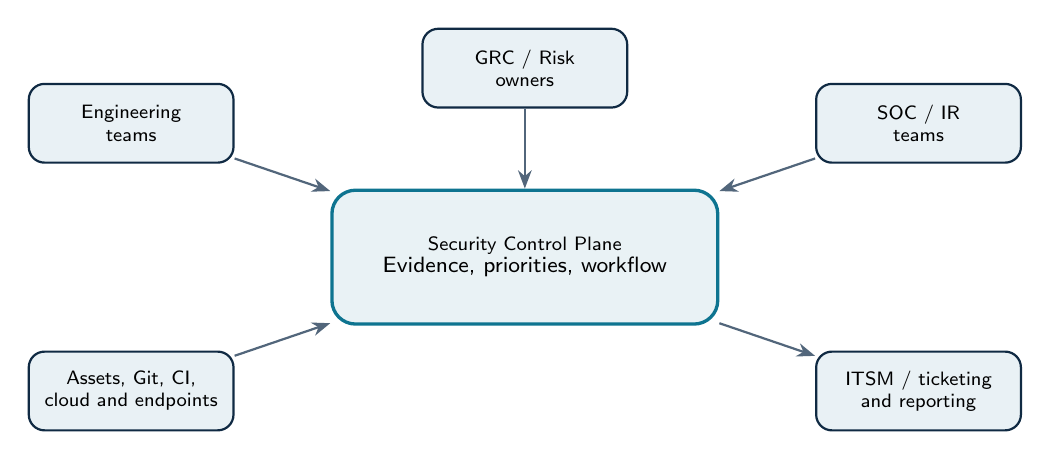
\begin{tikzpicture}[>=Stealth,node distance=10mm,font=\sffamily\scriptsize,
 role/.style={draw=navy,thick,rounded corners=2mm,fill=ice,minimum width=26mm,minimum height=10mm,align=center},
 core/.style={draw=cyan,very thick,rounded corners=3mm,fill=cyan!9,minimum width=49mm,minimum height=17mm,align=center},
 edge/.style={->,thick,draw=muted}]
\node[core] (platform) at (0,0) {Security Control Plane\\\footnotesize Evidence, priorities, workflow};
\node[role] (eng) at (-5,1.7) {Engineering\\teams};
\node[role] (soc) at (5,1.7) {SOC / IR\\teams};
\node[role] (risk) at (0,2.4) {GRC / Risk\\owners};
\node[role] (systems) at (-5,-1.7) {Assets, Git, CI,\\cloud and endpoints};
\node[role] (itsm) at (5,-1.7) {ITSM / ticketing\\and reporting};
\draw[edge] (eng) -- (platform);\draw[edge] (soc) -- (platform);\draw[edge] (risk) -- (platform);
\draw[edge] (systems) -- (platform);
\draw[edge] (platform) -- (itsm);
\end{tikzpicture}
\end{center}
\textbf{Trust boundary.} The control plane stores privileged vulnerability, identity and asset data. Scanner credentials, endpoint access and signing material reside in their own secure stores; the control plane uses least-privilege, auditable service identities.

\section{Container view and logical flows}
\begin{center}
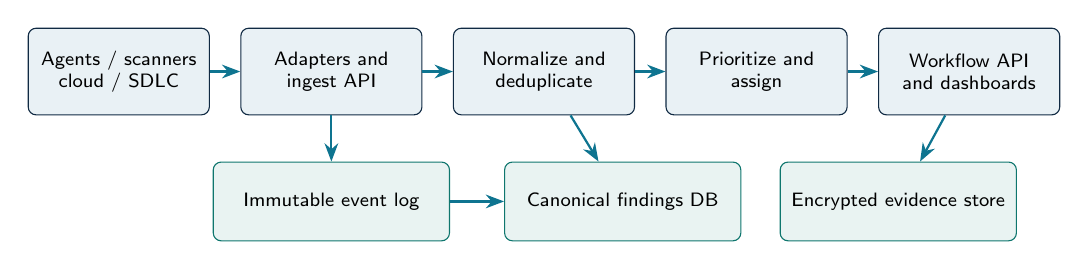
\begin{tikzpicture}[>=Stealth,font=\sffamily\scriptsize,
 block/.style={draw=navy,rounded corners=1mm,fill=ice,minimum width=23mm,minimum height=11mm,align=center},
 store/.style={draw=teal,rounded corners=1mm,fill=teal!9,minimum width=30mm,minimum height=10mm,align=center},
 flow/.style={->,thick,draw=cyan}]
\node[block] (sources) at (-5.4,0) {Agents / scanners\\cloud / SDLC};
\node[block] (ingest) at (-2.7,0) {Adapters and\\ingest API};
\node[block] (normal) at (0,0) {Normalize and\\deduplicate};
\node[block] (risk) at (2.7,0) {Prioritize and\\assign};
\node[block] (api) at (5.4,0) {Workflow API\\and dashboards};
\node[store] (events) at (-2.7,-1.65) {Immutable event log};
\node[store] (db) at (1.0,-1.65) {Canonical findings DB};
\node[store] (evidence) at (4.5,-1.65) {Encrypted evidence store};
\draw[flow] (sources)--(ingest);\draw[flow](ingest)--(normal);\draw[flow](normal)--(risk);\draw[flow](risk)--(api);
\draw[flow] (ingest)--(events);\draw[flow] (normal)--(db);\draw[flow] (api)--(evidence);
\draw[flow] (events)--(db);
\end{tikzpicture}
\end{center}
\textbf{Proposed (not verified native integrations):} ingestion over REST/webhook or batch import; a durable queue for retry and replay; PostgreSQL for authoritative workflow entities; object storage for evidence; optional scalable search/index service for telemetry. Do not use a SIEM index as the only system of record for approved risk decisions.

\section{Component view: findings service}

\noindent\begin{tabularx}{\textwidth}{P{0.23\textwidth}P{0.30\textwidth}Y}
\toprule Component & Responsibility & Design constraints\\\midrule
Connector registry & Source configuration and scopes & Typed credentials and egress allowlists\\
Parser/validator & Preserve raw payload and validate formats & Reject invalid SARIF/SBOM separately from processing results\\
Identity resolver & Bind repo, asset, project and environment & Explicit aliases, collision protection, audit history\\
Dedupe engine & Compute scoped stable fingerprints & Never merge unrelated tenants or distinct affected instances\\
Enrichment engine & CVE/CWE, EPSS, KEV, business exposure & Track feed date and absence; no opaque risk claims\\
Policy engine & SLA, exception and severity rules & Signed/versioned rules with accountable approvers\\
Remediation sync & Issue and workflow exchange & Idempotency, rate limits, backoff, dead-letter queues\\
Audit/evidence writer & Immutable history and forensic provenance & Encryption, legal hold, retention and access logging\\
\bottomrule
\end{tabularx}

\section{UML deployment-inspired view}
\begin{center}
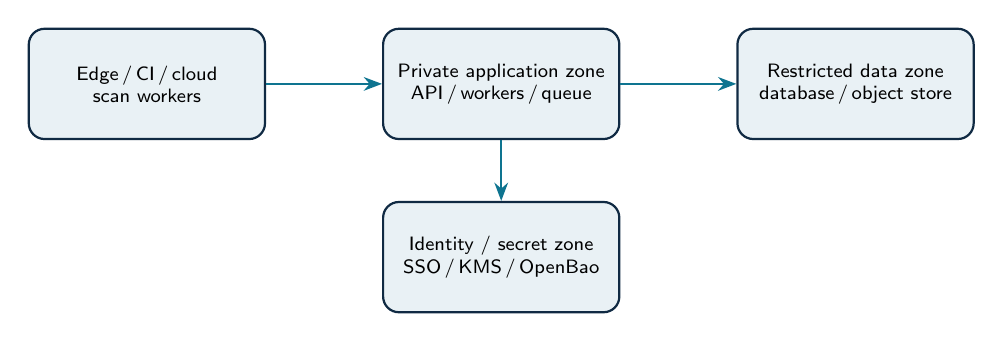
\begin{tikzpicture}[font=\sffamily\scriptsize,>=Stealth,
 device/.style={draw=navy,thick,fill=ice,rounded corners=2mm,minimum width=30mm,minimum height=14mm,align=center},
 connection/.style={->,line width=0.8pt,draw=cyan}]
\node[device] (edge) at (-4.5,1.1) {Edge\,/\,CI\,/\,cloud\\scan workers};
\node[device] (app) at (0,1.1) {Private application zone\\API\,/\,workers\,/\,queue};
\node[device] (db) at (4.5,1.1) {Restricted data zone\\database\,/\,object store};
\node[device] (auth) at (0,-1.1) {Identity / secret zone\\SSO\,/\,KMS\,/\,OpenBao};
\draw[connection] (edge)--(app);\draw[connection] (app)--(db);\draw[connection] (app)--(auth);
\end{tikzpicture}
\end{center}
\textbf{Deployment constraints:} private networks, egress control, audited service accounts, identity federation, object-store lifecycle controls, application secrets outside Git, tested failover, alerting on dropped events and queue growth, separate production/test security domains.

\section{Security entity identities and deduplication}

\noindent\begin{tabularx}{\textwidth}{P{0.19\textwidth}Y}
\toprule Entity & Identity / relationship\\\midrule
Asset & Stable source-specific and canonical asset IDs; may have host, cloud, device, repo or workload aliases.\\
Vulnerability & Public advisory/weakness identity (e.g. CVE/GHSA/CWE); not a proof a given asset is affected.\\
Finding & Source result on a particular asset/component, location and observation context; versioned over time.\\
Exposure & Validated reachable/affected condition tied to environment, compensating controls and owners.\\
Incident & Security event investigation that may reference many assets and findings.\\
Work item & Action with owner, due date, SLA, verification state and linked findings.\\
Risk decision & Approved exception with justification, expiry, evidence and accountable authority.\\
\bottomrule
\end{tabularx}
\textbf{Fingerprint concept:} \texttt{SHA-256(tenant || source || assetID || vulnerabilityID || location || ruleID)} using canonical, length-delimited representations, with merge exceptions for changing paths, aliases, and multi-source observations. Never rely on CVE alone as the deduplication key.

\section{Evidence normalization contracts}
Retain raw original SARIF, CycloneDX/SPDX, OSCAL, STIX, and scanner JSON in protected evidence storage. Parse to a separately versioned canonical model. For package vulnerabilities, prefer PURL with version/qualifiers, and maintain CPE mapping as corroborating evidence where applicable. Store enrichment timestamps for FIRST EPSS and CISA KEV; record negative/unknown states distinctly. Severity, exploitability, business criticality and vulnerability presence must remain separate fields.

\subsection{Illustrative canonical finding (custom platform contract)}
\begin{minted}{json}
{
  "schema_version": "1.0.0",
  "finding_id": "fnd-000001",
  "tenant_id": "tenant-001",
  "source": {"name": "ci-scan", "run_id": "run-123"},
  "asset": {"asset_id": "app-001", "environment": "staging"},
  "affected_component": {"purl": "pkg:maven/example/app@1.0.0"},
  "vulnerability": {"cve": null, "ghsa": null, "cwe": "CWE-89"},
  "assessment": {
    "cvss_base_score": null, "epss_probability": null,
    "epss_date": null, "cisa_kev": null,
    "reachability": "unknown", "business_criticality": "medium"
  },
  "workflow": {"status": "new", "owner": null, "due_date": null},
  "evidence": {"raw_object_uri": "s3://example-evidence/record.json"},
  "observed_at": "2026-10-12T12:00:00Z"
}
\end{minted}
\textit{Illustration only:} not an actual scanner result, live object-store URL, supported native API or upstream finding.

\subsection{Proposed integration API surface}

\noindent\begin{tabularx}{\textwidth}{P{0.31\textwidth}Y}
\toprule Custom route & Semantics\\\midrule
\texttt{POST /v1/ingestions} & Submit signed source envelopes with idempotency key; return async job reference.\\
\texttt{GET /v1/findings} & Filter scoped findings by owner, asset, severity, state and observation time.\\
\texttt{PATCH /v1/findings/\{id\}} & Validated workflow transition; enforce ETag or revision check.\\
\texttt{POST /v1/exceptions} & Request risk exception with approver, compensating controls and expiry.\\
\texttt{POST /v1/evidence} & Register immutable evidence and checksum with source provenance.\\
\texttt{GET /v1/health} & Readiness, ingestion lag, stale feeds and dependency health.\\
\bottomrule
\end{tabularx}
All endpoints are \textbf{proposed new APIs}. Require OAuth2/OIDC service identity, fine-grained authorization, rate limiting, detailed access audit, replay safeguards, and tenant-bound row-level authorization.

\chapter{Platform engineering and design contracts}
\section{Build versus integrate}
Most source functions should remain upstream products: do not recreate a SAST engine, DAST engine, vulnerability feed, SIEM, secrets backend, or CTI graph. Build bespoke services only for cross-source ownership, organization-specific risk decisions, portable evidence and the workflow connections that are not already available within a selected platform.

\noindent\begin{tabularx}{\textwidth}{P{0.23\textwidth}P{0.14\textwidth}Y}
\toprule Service & Decision & Requirement and acceptance result\\\midrule
Asset catalog & Integrate first & Reconcile authoritative owner, business service and technical aliases for 95\% of in-scope managed assets; missing owners reported, not silently defaulted.\\
Scanner coordinator & Integrate / thin service & Scheduled scope-bound jobs, concurrency limits, credential tenancy; 100\% scheduled runs accounted for as completed/failed/canceled.\\
Findings normalization & Build thin adapter tier & SARIF, SBOM and scanner adapters preserve raw artifact hashes and reject invalid schemas deterministically.\\
Prioritization & Build rules component & Transparent versioned policy, KEV/EPSS timestamped, manual override audited, no automatic false-positive dispositions.\\
Remediation workflows & Integrate ITSM first & Reconcile work-item state bi-directionally; retries must not create duplicate issues.\\
Exceptions and approvals & Integrate GRC or build & Request/review/expire decisions with accountable approver, expiry alert and historical audit record.\\
Security reports & Compose from sources & Traceable metrics with source, time window, denominator and freshness statement.\\
Admin console & Deferred & Only after existing UIs demonstrably fail multi-source workflow needs.\\
\bottomrule
\end{tabularx}
\section{Functional and nonfunctional requirements}
\begin{longtable}{P{0.15\textwidth}P{0.60\textwidth}P{0.17\textwidth}}
\toprule ID & Requirement / measurable acceptance & Owner\\\midrule\endfirsthead
\toprule ID & Requirement & Owner\\\midrule\endhead
FR-001 & Import at least one source each for endpoints, infrastructure vulnerabilities, CI SAST, secret scanning and SBOMs; preserve source timestamps. & Platform\\
FR-002 & Asset alias reconciliation shall preserve independent tenant and environment boundaries. & Asset team\\
FR-003 & Deduplicated issue creation shall be idempotent under replayed webhook messages. & Platform\\
FR-004 & Risk approval shall require reason, named approver, compensating controls, owner and expiration. & GRC\\
FR-005 & Mark ``fixed'' only after a supporting re-scan or documented manual verification. & AppSec\\
FR-006 & Preserve raw signed/hash-addressed evidence and immutable audit sequence for changes. & IR/GRC\\
FR-007 & Export canonical findings with evidence provenance in JSON and human-readable formats. & Platform\\
FR-008 & Alert on stale scanners, ingestion lag, connector auth failure, and expiring exceptions. & SOC\\
NFR-001 & Encrypt traffic and storage; use distinct short-lived scoped service identities. & IAM\\
NFR-002 & Backups must be tested in an isolated recovery environment against agreed RTO/RPO. & SRE\\
NFR-003 & Ingest handlers must enforce size limits, schema limits, retries, queue quotas and poison-message quarantine. & Platform\\
NFR-004 & Report lineage, extraction time and stale-feed status, including KEV/EPSS snapshots. & Analytics\\
NFR-005 & Define and load-test availability, peak EPS, mean ingest lag, and storage capacity targets for the actual tier. & SRE\\
NFR-006 & Require signed build artifacts, reproducible IaC deployment plan and dependency disclosure. & Supply chain\\
\bottomrule\end{longtable}
\section{Proposed reference engineering stack}
API layer: Python/FastAPI or Go; PostgreSQL for transactional findings and owner state; a durable message broker selected from an OSS-approved distribution; object storage with encrypted bucket/versioning/retention controls; OpenTelemetry Collector/Fluent Bit for suitable non-secret telemetry; version-controlled infrastructure using Terraform-compatible OSS tooling or OpenTofu; Ansible for systems automation; Kubernetes + GitOps only once complexity warrants it. The technical stack is a \emph{recommendation}, not a claim that selected security tools have native, certified connectors to every component.

\section{Transparent risk-triage sketch}
A sample queueing heuristic may combine normalized CVSS severity $C$, EPSS percentile $E$ (not a probability transformed arbitrarily), CISA KEV presence $K$, exposure $X$, and asset criticality $A$:
\[
P = 0.20 C + 0.25 E + 0.35 K + 0.10 X + 0.10 A,
\quad C,E,K,X,A \in [0,1].
\]
Treat the weights as a proposed policy subject to calibration, not a generally applicable scientific risk equation. Store original CVSS score/vector, EPSS probability and percentile separately, along with the score date. A public internet-facing KEV issue should generally receive expedited human review regardless of aggregate score. Validate exploitable paths and operating conditions; do not use generic numerical rankings to override safety-critical systems or approved risk tolerance.

\section{Architecture decisions and anti-patterns}
\begin{itemize}[leftmargin=1.4em]
\item \textbf{ADR-001:} Single normalized finding store, immutable raw artifacts: avoids evidence loss while supporting deduplication.
\item \textbf{ADR-002:} Existing identity and ITSM before new platforms: reduces administrative duplication and inconsistent state.
\item \textbf{ADR-003:} Scoped scanner identities and allowlists: avoids accidental third-party or production-impacting scans.
\item \textbf{ADR-004:} Queue-driven adapters: isolates scanner and ITSM availability, supports replay and durable delivery.
\item \textbf{ADR-005:} Compliance evidence is derived from observed systems, not self-asserted tool installation.
\item \textbf{ADR-006:} Preserve versioned schemas for assets, findings, risks and ownership independently.
\end{itemize}

\chapter{Deployment and operations runbooks}
\section{RB-01: establish and protect a management plane}
\begin{enumerate}[leftmargin=1.6em]
\item Identify production security operators, infrastructure owners and data custodians; classify sensitive logs and findings.
\item Provision isolated management networks, admin access via existing SSO/MFA, encryption keys, centralized time synchronization and restrictive outbound network policy.
\item Set up IaC and configuration code reviews; record secure base images, source revisions and artifact signatures.
\item Deploy a nonproduction integration environment with sanitized or synthetic data; verify authorization and tenant boundaries.
\item Configure encrypted backups before persisting authentic findings; perform an isolated restore exercise.
\item Record operational metrics: connector freshness, event rate, queue backlog, scanner age, storage growth, and backup status.
\end{enumerate}
\textbf{Exit gate:} documented recoverability, two-person privileged change approval, proof that unauthorized tenant queries fail, and an incident contact path.

\section{RB-02: onboard an inventory and scanner}
\begin{enumerate}[leftmargin=1.6em]
\item Obtain written target scope and owner authorization; identify asset IDs, environment and business ownership.
\item Create a source-specific service principal with read-only permissions when the workflow allows it.
\item Pin and verify the scanner's upstream release, license, policy content and dependencies.
\item Test on known benign fixtures or explicitly authorized staging assets; capture timestamps and raw evidence.
\item Configure transformation, normalization, duplicate-key rules and quarantine for invalid input.
\item Reconcile a sample of source results with normalized findings, work items and closed-loop remediation rechecks.
\item Publish run frequency, quota, false-positive review procedure and escalation ownership.
\end{enumerate}
\textbf{Exit gate:} proven input-to-evidence lineage, no duplicate tickets during event replay, and documented permission boundaries.

\section{RB-03: secure CI/CD adoption}
In a controlled branch: run Gitleaks as a pre-merge secret gate, Semgrep OSS with curated rule sets for supported languages, an image/dependency scanner, and Syft to generate a CycloneDX or SPDX SBOM. Upload an SBOM into a controlled portfolio analysis platform where supported. Perform safe staging DAST only against permitted endpoints and dedicated test credentials. Add Cosign signatures and verifications at the release boundary. Treat all illustrative CLI steps as pseudo-workflow until exact tool options are checked against a pinned release.
\begin{minted}{yaml}
# Pseudocode: CI orchestrator stages (not product CLI syntax)
stages:
  - verify-source-and-dependencies
  - detect-secrets-and-static-flaws
  - produce-and-validate-sbom
  - inspect-artifacts-and-config
  - sign-and-publish-attestations
  - sync-owned-findings
  - evaluate-release-policy
\end{minted}
\textbf{Quality gates:} zero exposed credentials, reproducible evidence, documented scanner failure semantics, false-positive adjudication by owner, and an explicit exception pathway.

\section{RB-04: detection and incident escalation}
Security Operations maintains named playbooks for ransomware, credential exposure, cloud IAM abuse, web application compromise and backup tampering. Each playbook specifies triage identity, severity criteria, evidence acquisition constraints, containment approval, communication authority and chain of custody. Simulate a harmless test indicator first, confirm end-to-end routing, then tune false positives and retention. Irreversible containment requires explicit human authorization unless a formally approved automated response policy exists.

\section{RB-05: upgrade and rollback}
Before upgrades, confirm release provenance, migration notes, schema compatibility, backup integrity, deployment health and vendor/plugin constraints. Apply changes in staging, run functional and security regression tests, and document database backward-compatibility. For high-risk migrations, prefer blue/green or controlled canary rollout and an exercise-tested rollback plan. A successful package installation is not proof the product has resumed effective detection.

\section{RB-06: recovery drill}
At least quarterly, choose a representative protected dataset; restore to an isolated environment using the documented procedures; verify decrypted data integrity, key availability and application dependencies; record actual recovery time and recovery point; update deficiencies and repeat failed controls. Frequency is a proposed default and should be adapted to agreed recovery objectives and regulation.

\section{Minimum handoff evidence pack}

\noindent\begin{tabularx}{\textwidth}{P{0.24\textwidth}Y}
\toprule Artifact & Required content\\\midrule
Architecture decision log & Accepted tradeoffs, rejected alternatives, impact assessment and owners.\\
Tool qualification sheet & Verified version, license, SBOM, security policy, edition, installation path.\\
Access review & Human/service RBAC, secret rotation, privileged access tests.\\
Operational SLOs & Collection freshness, ingestion lag, dashboard availability, alert accuracy.\\
Recovery evidence & Backup age, restoration test, measured RTO/RPO, corrective actions.\\
Detection test pack & Safe fixtures, expected alert classification, test timestamp and result.\\
Security case records & Provenance, owner, state changes, exception approvals, remediation validation.\\
\bottomrule
\end{tabularx}

\chapter{Implementation roadmap and work backlog}
\section{Prerequisite-driven delivery sequence}
The sequence below is one valid topological order for the proposed dependency graph. Work packages can overlap when the engineering dependency is satisfied; time bands are planning windows, not promises. Estimates refer to \emph{engineer-days} of direct effort for initial configuration or integration and exclude approvals, hiring, procurement, and major migrations.
\begin{center}
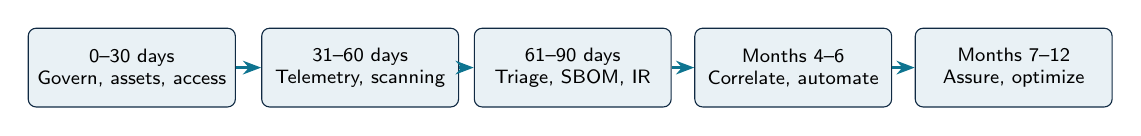
\begin{tikzpicture}[font=\sffamily\scriptsize,>=Stealth,stagebox/.style={draw=navy,rounded corners=1mm,fill=ice,minimum width=25mm,minimum height=10mm,align=center},conn/.style={->,draw=cyan,thick}]
\node[stagebox] (a) at (-5.6,0) {0--30 days\\Govern, assets, access};
\node[stagebox] (b) at (-2.7,0) {31--60 days\\Telemetry, scanning};
\node[stagebox] (c) at (0,0) {61--90 days\\Triage, SBOM, IR};
\node[stagebox] (d) at (2.8,0) {Months 4--6\\Correlate, automate};
\node[stagebox] (e) at (5.6,0) {Months 7--12\\Assure, optimize};
\draw[conn] (a)--(b);\draw[conn](b)--(c);\draw[conn](c)--(d);\draw[conn](d)--(e);
\end{tikzpicture}
\end{center}
\small
\begin{longtable}{P{0.09\textwidth}P{0.275\textwidth}P{0.12\textwidth}P{0.135\textwidth}P{0.105\textwidth}P{0.07\textwidth}}
\toprule ID & Work package & Window & Depends on & Owner & Days\\\midrule\endfirsthead
\toprule ID & Work package & Window & Depends on & Owner & Days\\\midrule\endhead

WP-01 & Risk mandate and asset owners & 0–30 & None & GRC & 5–10 \\
WP-02 & Security program access and MFA & 0–30 & WP-01 & IAM & 5–10 \\
WP-03 & Asset + application inventory & 0–30 & WP-01 & Infra & 10–20 \\
WP-04 & Recovery targets and baseline backup & 0–30 & WP-01,03 & SRE & 8–16 \\
WP-05 & Centralize audit log sources & 31–60 & WP-02,03 & SOC & 10–20 \\
WP-06 & Managed patch and config control & 31–60 & WP-03 & Infra & 10–20 \\
WP-07 & Credential-safe scanner scope & 31–60 & WP-02,03 & Vuln & 5–10 \\
WP-08 & Repository security CI & 31–60 & WP-02,03 & AppSec & 10–20 \\
WP-09 & Infra vulnerability baseline & 61–90 & WP-03,07 & Vuln & 10–20 \\
WP-10 & SBOM and dependency inventory & 61–90 & WP-08 & AppSec & 7–15 \\
WP-11 & Detection content and triage & 61–90 & WP-05 & SOC & 10–20 \\
WP-12 & Incident and restore exercise & 61–90 & WP-04,11 & IR/SRE & 6–12 \\
WP-13 & Finding normalization prototype & 4–6 months & WP-03,09,10 & Platform & 15–30 \\
WP-14 & Owned remediation and ITSM sync & 4–6 months & WP-13 & Vuln/ITSM & 10–25 \\
WP-15 & Cloud posture integration & 4–6 months & WP-03,07 & CloudSec & 8–16 \\
WP-16 & K8s policy and runtime pilot & 4–6 months & WP-15 & Platform & 10–22 \\
WP-17 & Evidence/exception automation & 4–6 months & WP-13,14 & GRC & 10–18 \\
WP-18 & CTI and DFIR targeted deployment & 7–12 months & WP-11,12,13 & SOC/IR & 10–25 \\
WP-19 & Supply chain provenance gate & 7–12 months & WP-10,16 & AppSec & 10–20 \\
WP-20 & Purple team and executive metrics & 7–12 months & WP-11,14,17 & SOC/GRC & 12–24 \\
\bottomrule\end{longtable}\normalsize
\section{Work-package validation and handoff}
\begin{longtable}{P{0.1\textwidth}P{0.60\textwidth}P{0.19\textwidth}}
\toprule ID & Acceptance criterion & Delivery risk\\\midrule\endfirsthead
\toprule ID & Acceptance & Risk\\\midrule\endhead

WP-01 & Approved scope, risk appetite, owners; handoff includes operational owner and runbook & Limited personnel and integration effort \\
WP-02 & Admin MFA + least-privilege review; handoff includes operational owner and runbook & Limited personnel and integration effort \\
WP-03 & Owned records and reconciliation; handoff includes operational owner and runbook & Limited personnel and integration effort \\
WP-04 & Isolated restore succeeds; handoff includes operational owner and runbook & Limited personnel and integration effort \\
WP-05 & Critical source list + event health; handoff includes operational owner and runbook & Limited personnel and integration effort \\
WP-06 & Exception and drift metrics; handoff includes operational owner and runbook & Limited personnel and integration effort \\
WP-07 & Authorized staging profile; handoff includes operational owner and runbook & Limited personnel and integration effort \\
WP-08 & Validated findings on test repo; handoff includes operational owner and runbook & Limited personnel and integration effort \\
WP-09 & Confirmed asset-bound findings; handoff includes operational owner and runbook & Data quality, access and scope creep \\
WP-10 & Versioned SBOM and import evidence; handoff includes operational owner and runbook & Data quality, access and scope creep \\
WP-11 & Safe rule trigger and escalation; handoff includes operational owner and runbook & Data quality, access and scope creep \\
WP-12 & Tabletop + technical recovery evidence; handoff includes operational owner and runbook & Data quality, access and scope creep \\
WP-13 & Source lineage; schema contract; handoff includes operational owner and runbook & Data quality, access and scope creep \\
WP-14 & Replay without duplicate issues; handoff includes operational owner and runbook & Data quality, access and scope creep \\
WP-15 & Cloud ownership and drift findings; handoff includes operational owner and runbook & Data quality, access and scope creep \\
WP-16 & Fail-safe policy tests; handoff includes operational owner and runbook & Data quality, access and scope creep \\
WP-17 & Approved expiring exceptions; handoff includes operational owner and runbook & Data quality, access and scope creep \\
WP-18 & Measured enrichment/use case; handoff includes operational owner and runbook & Data quality, access and scope creep \\
WP-19 & Release artifact verification; handoff includes operational owner and runbook & Data quality, access and scope creep \\
WP-20 & Control validation and KPIs; handoff includes operational owner and runbook & Data quality, access and scope creep \\
\bottomrule\end{longtable}
\section{Minimum viable platform acceptance}
The initial 90-day minimum comprises WP-01 through WP-12 with documented risk ownership, inventory and identities, successful restore, protected telemetry, authorized scan cadence, software CI controls where applicable, and human incident escalation. WP-13 onward builds central orchestration and correlation only after the sources and identity model work reliably.

\section{Engineering backlog hierarchy}

\noindent\begin{tabularx}{\textwidth}{P{0.24\textwidth}Y}
\toprule Epic & Features and nonfunctional acceptance themes\\\midrule
EP-01 Control foundation & Asset linkage, identity least privilege, policy mapping, recovery controls; FR-002 / NFR-001 / NFR-002.\\
EP-02 Secure delivery & Secret scanning, SAST, SBOM, DAST staging, provenance; FR-001 / FR-005 / NFR-006.\\
EP-03 Detection and response & Telemetry collectors, detection-as-code, incident case linkage, forensic evidence; FR-006 / FR-008.\\
EP-04 Unified exposure & Findings schema, deduplication, enrichment, exception lifecycle, remediation sync; FR-002--004.\\
EP-05 Assurance & Restore validation, compliance evidence, risk KPIs, adversary testing; FR-007 / NFR-004--005.\\
\bottomrule
\end{tabularx}

\chapter{Cost, staffing and operational sustainability}
\section{Total-cost model}
Open-source license fees can be zero while infrastructure, retention, staff, response coverage, security engineering, and recovery generate material expense. For each tier model:
\[
C_{annual}=12(C_{compute}+C_{storage}+C_{network}+C_{support})
 + H_{staff}\cdot R_{loaded}+C_{training}+C_{migration}.
\]
The model excludes business losses from incidents; prices are \emph{illustrative assumptions}, not quotes, sourced rate cards or vendor pricing.

\section{Scenario assumptions and annual planning ranges}

\noindent\begin{tabularx}{\textwidth}{P{0.19\textwidth}YYY}
\toprule Variable & Tier 1 / small & Tier 2 / growing & Tier 3 / complex\\\midrule
Managed assets (assumed) & 25--150 & 150--2,000 & 2,000--25,000+\\
Retention baseline & 30--90 days & 90--180 days & 180--365+ days\\
Engineering time & 0.25--0.75 FTE & 1.5--4 FTE & 5--15+ FTE\\
Infrastructure / year & \$2k--\$15k & \$20k--\$120k & \$150k--\$1.2m+\\
Loaded staff rate/year & \$160k (example) & \$160k (example) & \$160k (example)\\
Approx total/year & \$42k--\$135k & \$260k--\$760k & \$950k--\$3.6m+\\
\bottomrule
\end{tabularx}
\textit{Interpretation:} envelopes are coarse examples from assumed scale, deployment topology and staffing, not surveyed market averages. The tier total ranges are independently rounded; they are not budget commitments. Existing IAM/EDR/SIEM commitments, self-hosted vs cloud, managed operations, OT safety constraints, and labor markets can change the result substantially. Validate with local utilization and loaded labor rates.

\section{Telemetry capacity example}
At a hypothetical 1,000 events/second, 700 bytes/event average, 90 days retention, a 1.8 indexing/compression/metadata multiplier and 2 replicated copies:
\[
V \approx \frac{1000\cdot700\cdot86400\cdot90\cdot1.8\cdot2}{10^{12}}
\approx 19.6\ \text{TB}.
\]
This is an \emph{illustrative raw planning approximation}, not a hardware recommendation. Actual compression, shards, peak burst rates, replicas, warm/cold tiers and searchable data vary by architecture. Test sustained event size and index amplification on representative source logs.

\section{Sustainability gates}
\begin{enumerate}[leftmargin=1.6em]
\item Check release recency, reproducible builds, signed artifacts, repository maintainers, disclosure process and outstanding security regressions.
\item Review support dependency and changes in community versus enterprise licensing or commercial feature allocation.
\item Require a staffed patching and recovery plan for every stateful component.
\item Budget rule/indicator content management separately from the detection engine.
\item Prevent single maintainer or sole integrator knowledge from becoming an operational single point of failure.
\end{enumerate}
\section{Key executive indicators}
Report asset ownership coverage, active scanning coverage, open/aged findings by verified severity and business exposure, KEV remediation age, mean time to validate remediation, secret exposure response, rule test pass rate, failed ingestion jobs, stale evidence rate, expired exceptions, recoverability test success and security platform uptime. Always disclose denominators, time period and exclusions.

\chapter{Tool registry schema and reproducibility}
\section{Record-level metadata contract}
The supplied machine-readable registry contains 140 records, an evidence state and extensive placeholders for evidence not verified in this review. Each record has identifiers, capability mapping, upstream references, license scope, research status, deployability and security risk review fields. Text values such as \texttt{Not verified} should become typed \texttt{null} with an explicit status field in production pipelines; the current human-readable format intentionally makes missing verification visible.

\begin{minted}{json}
{
  "$schema": "https://json-schema.org/draft/2020-12/schema",
  "type": "object",
  "required": ["id", "name", "domain", "repository_url",
               "license_class", "research_status", "evidence"],
  "properties": {
    "id": {"type": "string", "pattern": "^TOOL-[0-9]{3,}$"},
    "name": {"type": "string", "minLength": 2},
    "domain": {"type": "string", "minLength": 2},
    "repository_url": {"type": "string", "format": "uri"},
    "license_class": {
      "enum": ["OSS", "OSS (component-scope review)",
               "Open Core", "Source Available", "Freeware",
               "Commercial", "Unverified"]
    },
    "research_status": {
      "enum": ["Upstream reviewed", "Discovery candidate only"]
    },
    "evidence": {"type": "array", "items": {"type": "string", "format": "uri"}},
    "verification_date": {"type": "string", "format": "date"}
  },
  "additionalProperties": true
}
\end{minted}
The full repository registry also includes fields for version, upstream release date, last maintenance observation, platforms, authentication, interfaces, support, restrictions, technical limitations, alternate tools, confidence, and verification state. A production JSON Schema should be generated separately with explicit field types, enumerations, controlled nullability and migrations.

\section{Validation rules}
\begin{enumerate}[leftmargin=1.6em]
\item Require stable unique \texttt{TOOL-*} IDs; reject duplicate project names or source repository identities after canonicalization.
\item Validate URLs, license expressions against SPDX where applicable, and license/edition claims against source evidence.
\item Require source timestamps and immutable links for licensed/ranked selections; missing data remains unresolved.
\item Automatically flag projects with no observed security policy, discontinued support, or releases beyond the organization's approved recency tolerance.
\item Reject the use of \texttt{Discovery candidate only} products in a strict production allowlist; escalate open-core or mixed-license selections to legal and platform owners.
\item Re-check license and security metadata at every selected-version change and at a defined periodic cadence.
\end{enumerate}
\section{Reproduction commands}
\begin{minted}{bash}
# Build the editable LaTeX report from the included generator:
python3 build_report.py

# Compile the standalone LaTeX report (pdfLaTeX, Type 1 fonts):
latexmk -pdf -interaction=nonstopmode \
  -halt-on-error -outdir=. enterprise_oss_security.tex

# Validate the registry's parseability:
python3 -m json.tool tool_registry.json >/dev/null
\end{minted}
\textbf{Deliverables included in the package:} \texttt{enterprise\_oss\_security.tex}, \texttt{enterprise\_oss\_security.pdf}, \texttt{tool\_registry.json}, \texttt{tool\_catalog.csv}, \texttt{tool\_catalog.md}, and the source generator. The generated report is self-contained; an Internet connection is not required to compile it.

\chapter{Quality assurance, residual gaps and next actions}
\section{Research assurance checklist}

\noindent\begin{tabularx}{\textwidth}{P{0.39\textwidth}P{0.14\textwidth}Y}
\toprule Objective & State & Evidence / residual work\\\midrule
All 28 source category landings opened & Observed & 28 site category pages reviewed; counts taken from site.\\
Source inventory complete to profile level & Incomplete & 337 advertised, individual profile audit not executed.\\
Broad multi-domain tool candidate catalog & Complete (discovery) & 140 unique entries, 24 upstream-reviewed, 116 further leads.\\
Current release and activity for every tool & Incomplete & Latest stable tags/dates generally unverified.\\
License and edition validation for all candidates & Incomplete & Verified shortlist only; many feature/plugin/feed exceptions outstanding.\\
Enterprise control capability architecture & Proposed & 28 defined capability contracts and maturity-sensitive adoption.\\
CSF/CIS and SDLC overlays & Proposed & Control-family mappings only; no asserted safeguard-level audit.\\
Tool ranking with traceable fit assumptions & Partial & Scenario scores labeled hypothetical; empirical PoC required.\\
Three reference deployment models & Proposed & Tier 1--3 specifications, ownership and security gates.\\
Integration design and format lineage & Proposed & Canonical finding model, API contracts and architectural views.\\
Runbook and work-package design & Proposed & Six procedures; 20 dependencies and acceptance criteria.\\
Total-cost analysis & Illustrative & Explicit assumptions; not a price quote.\\
\bottomrule
\end{tabularx}

\section{Priority unresolved investigations}
\begin{enumerate}[leftmargin=1.6em]
\item Individually inspect the directory's advertised profiles to establish a complete source snapshot with provenance and stable IDs.
\item Finish upstream license/edition/security reviews for the remaining 116 discovery candidates and confirm 2026 stable releases.
\item Verify tool APIs, authentication and data formats using exact versions for the deployment shortlist; create contract tests.
\item Validate control-by-control CIS IG and NIST CSF mappings against licensed authoritative source material.
\item Run an isolated proof of concept with one integration route per data family and collect operational measurements.
\item Confirm legal requirements, retention, data sovereignty, vendor support and service continuity for the target enterprise.
\item Establish budget from real cloud rates, telemetry workloads, labor assumptions and support commitments.
\end{enumerate}
\section{Recommended next engineering decisions}
Approve scope and minimum baseline; nominate a single owner for asset identities and a single owner for remediation state; qualify the 24 upstream-reviewed shortlist against intended artifacts/versions; define source-to-finding test fixtures; validate a three-source pilot (e.g., secrets/SAST, dependency SBOM and infrastructure vulnerabilities) with event replay and exception workflows; expand only after the pilot achieves dependable evidence quality and recovery.

\begin{caution}
\textbf{Safety and legal boundary.} Discovery and tool-selection research do not grant authorization to scan or exploit a website, cloud account, network or application. Perform active scans, credential testing, fuzzing and adversary simulation only against owned systems, approved laboratories or targets covered by explicit documented permission and controlled windows.
\end{caution}

\begin{thebibliography}{99}
\addcontentsline{toc}{chapter}{References and primary sources}

\bibitem{immunity} ImmunitySec. \emph{Software and tools directory}. \url{https://www.immunitysec.com/}. Accessed 2026-10-12.
\bibitem{nist} NIST. \emph{Cybersecurity Framework 2.0 (CSF Core)}. \url{https://www.nist.gov/cyberframework}. Accessed 2026-10-12.
\bibitem{cis} Center for Internet Security. \emph{CIS Controls v8.1 Implementation Groups}. \url{https://www.cisecurity.org/controls/implementation-groups}. Accessed 2026-10-12.
\bibitem{ssdf} NIST. \emph{Secure Software Development Framework, SP 800-218}. \url{https://csrc.nist.gov/pubs/sp/800/218/final}. Accessed 2026-10-12.
\bibitem{samm} OWASP. \emph{Software Assurance Maturity Model}. \url{https://owaspsamm.org/}. Accessed 2026-10-12.
\bibitem{asvs} OWASP. \emph{Application Security Verification Standard}. \url{https://owasp.org/www-project-application-security-verification-standard/}. Accessed 2026-10-12.
\bibitem{attack} MITRE. \emph{ATT\&CK knowledge base}. \url{https://attack.mitre.org/}. Accessed 2026-10-12.
\bibitem{atlas} MITRE. \emph{ATLAS AI threat knowledge base}. \url{https://atlas.mitre.org/}. Accessed 2026-10-12.
\bibitem{kev} CISA. \emph{Known Exploited Vulnerabilities catalog}. \url{https://www.cisa.gov/known-exploited-vulnerabilities-catalog}. Accessed 2026-10-12.
\bibitem{epss} FIRST. \emph{Exploit Prediction Scoring System}. \url{https://www.first.org/epss/}. Accessed 2026-10-12.
\bibitem{spdx} SPDX. \emph{Open standard for software bill of materials}. \url{https://spdx.dev/}. Accessed 2026-10-12.
\bibitem{cyclonedx} OWASP. \emph{CycloneDX software transparency standard}. \url{https://cyclonedx.org/}. Accessed 2026-10-12.
\bibitem{sarif} OASIS. \emph{Static Analysis Results Interchange Format}. \url{https://www.oasis-open.org/committees/sarif/}. Accessed 2026-10-12.
\bibitem{oscal} NIST. \emph{Open Security Controls Assessment Language}. \url{https://pages.nist.gov/OSCAL/}. Accessed 2026-10-12.
\bibitem{osi} Open Source Initiative. \emph{Approved open-source licenses}. \url{https://opensource.org/licenses}. Accessed 2026-10-12.
\bibitem{nmap} Nmap. \emph{NPSL source licensing}. \url{https://nmap.org/npsl/}. Accessed 2026-10-12.
\bibitem{greenbone} Greenbone. \emph{OpenVAS scanner: repository and license scope}. \url{https://github.com/greenbone/openvas-scanner}. Accessed 2026-10-12.
\bibitem{opencti} OpenCTI. \emph{Community and enterprise edition license information}. \url{https://github.com/OpenCTI-Platform/opencti}. Accessed 2026-10-12.
\bibitem{velociraptor} Velocidex. \emph{Velociraptor source license}. \url{https://github.com/Velocidex/velociraptor/blob/master/LICENSE}. Accessed 2026-10-12.
\bibitem{dependencytrack} OWASP Dependency-Track. \emph{Project repository and version migration notes}. \url{https://github.com/DependencyTrack/dependency-track}. Accessed 2026-10-12.
\bibitem{defectdojo} DefectDojo. \emph{Community repository and license}. \url{https://github.com/DefectDojo/django-DefectDojo}. Accessed 2026-10-12.
\bibitem{semgrep} Semgrep. \emph{Semgrep engine repository and copyright}. \url{https://github.com/semgrep/semgrep}. Accessed 2026-10-12.
\bibitem{restic} restic. \emph{Backup utility and source license}. \url{https://github.com/restic/restic}. Accessed 2026-10-12.
\end{thebibliography}
\appendix
\chapter{Source directory category links}
The following landing-page links correspond to the 28 category names examined. Category counts originate from the ImmunitySec index; individual upstream projects must be validated independently.

\noindent\textbf{AI Security Tools (10)} \hfill \url{https://www.immunitysec.com/ai-security/}\par
\noindent\textbf{Application Security Tools (23)} \hfill \url{https://www.immunitysec.com/appsec/}\par
\noindent\textbf{Binary Exploitation (7)} \hfill \url{https://www.immunitysec.com/binary-exploitation/}\par
\noindent\textbf{Cloud Security Tools (20)} \hfill \url{https://www.immunitysec.com/cloud-native-security/}\par
\noindent\textbf{CTF \& Practice Labs (16)} \hfill \url{https://www.immunitysec.com/ctf-labs/}\par
\noindent\textbf{Data Security Software (10)} \hfill \url{https://www.immunitysec.com/data-security/}\par
\noindent\textbf{Digital Forensics (12)} \hfill \url{https://www.immunitysec.com/dfir/}\par
\noindent\textbf{Email Security Software (13)} \hfill \url{https://www.immunitysec.com/email-security/}\par
\noindent\textbf{Fuzzing (10)} \hfill \url{https://www.immunitysec.com/fuzzing/}\par
\noindent\textbf{GRC Software (11)} \hfill \url{https://www.immunitysec.com/grc/}\par
\noindent\textbf{Honeypot \& Deception Tools (8)} \hfill \url{https://www.immunitysec.com/honeypots/}\par
\noindent\textbf{IAM Tools (10)} \hfill \url{https://www.immunitysec.com/iam/}\par
\noindent\textbf{Malware Analysis Tools (12)} \hfill \url{https://www.immunitysec.com/malware-analysis/}\par
\noindent\textbf{Mobile Security Software (8)} \hfill \url{https://www.immunitysec.com/mobile-security/}\par
\noindent\textbf{Network Monitoring Tools (5)} \hfill \url{https://www.immunitysec.com/network-monitoring/}\par
\noindent\textbf{Network Security Tools (13)} \hfill \url{https://www.immunitysec.com/network-security/}\par
\noindent\textbf{Open Source Intelligence Tools (19)} \hfill \url{https://www.immunitysec.com/osint/}\par
\noindent\textbf{OT/ICS Security Tools (6)} \hfill \url{https://www.immunitysec.com/ot-security/}\par
\noindent\textbf{Password Cracking (7)} \hfill \url{https://www.immunitysec.com/password-cracking/}\par
\noindent\textbf{Penetration Testing Tools (21)} \hfill \url{https://www.immunitysec.com/penetration-testing/}\par
\noindent\textbf{Phishing Simulation Tools (5)} \hfill \url{https://www.immunitysec.com/social-engineering/}\par
\noindent\textbf{Red Teaming Tools (11)} \hfill \url{https://www.immunitysec.com/red-team/}\par
\noindent\textbf{Reverse Engineering (12)} \hfill \url{https://www.immunitysec.com/reverse-engineering/}\par
\noindent\textbf{SIEM Tools (29)} \hfill \url{https://www.immunitysec.com/detection-engineering/}\par
\noindent\textbf{Software Composition Analysis Tools (12)} \hfill \url{https://www.immunitysec.com/supply-chain-security/}\par
\noindent\textbf{Threat Intelligence Tools (9)} \hfill \url{https://www.immunitysec.com/threat-intelligence/}\par
\noindent\textbf{Vulnerability Scanning (8)} \hfill \url{https://www.immunitysec.com/vulnerability-scanning/}\par
\noindent\textbf{Wireless \& RF Security (10)} \hfill \url{https://www.immunitysec.com/wireless-security/}\par
\chapter{Reviewed project evidence}
The following upstream project repositories were opened or used as primary license or capabilities evidence during this review. A reviewed repository is not an assertion that its latest release, full bill of materials, or every advertised feature was audited.

\noindent\textbf{ZAP} \hfill \url{https://github.com/zaproxy/zaproxy}\par
\noindent\textbf{Semgrep OSS engine} \hfill \url{https://github.com/semgrep/semgrep}\par
\noindent\textbf{Gitleaks} \hfill \url{https://github.com/gitleaks/gitleaks}\par
\noindent\textbf{Trivy} \hfill \url{https://github.com/aquasecurity/trivy}\par
\noindent\textbf{Syft} \hfill \url{https://github.com/anchore/syft}\par
\noindent\textbf{Grype} \hfill \url{https://github.com/anchore/grype}\par
\noindent\textbf{Dependency-Track} \hfill \url{https://github.com/DependencyTrack/dependency-track}\par
\noindent\textbf{DefectDojo} \hfill \url{https://github.com/DefectDojo/django-DefectDojo}\par
\noindent\textbf{Keycloak} \hfill \url{https://github.com/keycloak/keycloak}\par
\noindent\textbf{OpenBao} \hfill \url{https://github.com/openbao/openbao}\par
\noindent\textbf{Wazuh} \hfill \url{https://github.com/wazuh/wazuh}\par
\noindent\textbf{Suricata} \hfill \url{https://github.com/OISF/suricata}\par
\noindent\textbf{Zeek} \hfill \url{https://github.com/zeek/zeek}\par
\noindent\textbf{Prowler} \hfill \url{https://github.com/prowler-cloud/prowler}\par
\noindent\textbf{Falco} \hfill \url{https://github.com/falcosecurity/falco}\par
\noindent\textbf{Kyverno} \hfill \url{https://github.com/kyverno/kyverno}\par
\noindent\textbf{Cosign} \hfill \url{https://github.com/sigstore/cosign}\par
\noindent\textbf{restic} \hfill \url{https://github.com/restic/restic}\par
\noindent\textbf{MISP} \hfill \url{https://github.com/MISP/MISP}\par
\noindent\textbf{OpenCTI Community} \hfill \url{https://github.com/OpenCTI-Platform/opencti}\par
\noindent\textbf{Greenbone OpenVAS Scanner} \hfill \url{https://github.com/greenbone/openvas-scanner}\par
\noindent\textbf{Velociraptor} \hfill \url{https://github.com/Velocidex/velociraptor}\par
\noindent\textbf{Open Policy Agent} \hfill \url{https://github.com/open-policy-agent/opa}\par
\noindent\textbf{osquery} \hfill \url{https://github.com/osquery/osquery}\par
\end{document}

